\documentclass[conference]{IEEEtran}
\IEEEoverridecommandlockouts
% The preceding line is only needed to identify funding in the first footnote. If that is unneeded, please comment it out.
%Template version as of 6/27/2024
\usepackage{pgfplots}  % Add this to use the axis environment
\pgfplotsset{compat=1.18}  % Ensures compatibility with the latest version



\usepackage{amsmath,amssymb,amsfonts}
\usepackage{algorithmic}
\usepackage{graphicx}
\usepackage{textcomp}
\usepackage{xcolor}
\usepackage{tabularx} % For extended tables
\usepackage[table]{xcolor} % For coloring tables
\usepackage{tikz}
\usetikzlibrary{trees, mindmap, shapes.geometric, positioning, fit, shapes.geometric, arrows, positioning, decorations.pathreplacing, calc}
\usepackage[backend=biber, style=ieee]{biblatex}  % Use biblatex with IEEE style
\addbibresource{myrefBibLaTeX.bib} 
\usepackage{pgfplotstable}


\begin{document}

\title{Challenges and Proposals on Using LLM Gen AI for Financial Risk Analysis *\\
{\footnotesize \textsuperscript{*}Note: Sub-titles are not captured for https://ieeexplore.ieee.org  and
should not be used}
\thanks{Identify applicable funding agency here. If none, delete this.}
}

\author{\IEEEauthorblockN{1\textsuperscript{st} Shivgan Joshi}
\IEEEauthorblockA{\textit{QcFinance IN} \\
\textit{name of organization (of Aff.)}\\
City, Country \\
email address or ORCID}
\and
\IEEEauthorblockN{2\textsuperscript{nd} Given Name Surname}
\IEEEauthorblockA{\textit{dept. name of organization (of Aff.)} \\
\textit{name of organization (of Aff.)}\\
City, Country \\
email address or ORCID}
\and
\IEEEauthorblockN{3\textsuperscript{rd} Given Name Surname}
\IEEEauthorblockA{\textit{dept. name of organization (of Aff.)} \\
\textit{name of organization (of Aff.)}\\
City, Country \\
email address or ORCID}
\and
\IEEEauthorblockN{4\textsuperscript{th} Given Name Surname}
\IEEEauthorblockA{\textit{dept. name of organization (of Aff.)} \\
\textit{name of organization (of Aff.)}\\
City, Country \\
email address or ORCID}
\and
\IEEEauthorblockN{5\textsuperscript{th} Given Name Surname}
\IEEEauthorblockA{\textit{dept. name of organization (of Aff.)} \\
\textit{name of organization (of Aff.)}\\
City, Country \\
email address or ORCID}
\and
\IEEEauthorblockN{6\textsuperscript{th} Given Name Surname}
\IEEEauthorblockA{\textit{dept. name of organization (of Aff.)} \\
\textit{name of organization (of Aff.)}\\
City, Country \\
email address or ORCID}
}

\maketitle

\begin{abstract}
In this paper we have proposed and demonstrated a protype on how to use GenAI in modeling Financial Risk Analysis.

Model development, validation and approval is an art and science. Mathematical models without human oversight can lead to failure. In this research we will look at how to use the current development in GenAi LLM to risk modeling.

This document is a model and instructions for \LaTeX.
This and the IEEEtran.cls file define the components of your paper [title, text, heads, etc.]. *CRITICAL: Do Not Use Symbols, Special Characters, Footnotes, 
or Math in Paper Title or Abstract.
\end{abstract}

\begin{IEEEkeywords}
Gen AI, Financial Risk, style, styling, insert.
\end{IEEEkeywords}

\section{Introduction}
A lot of information about risk modeling is already in public domains and ChatGPT kind of tools already have them in their models.
There are two ways to develop models, either use Open AI and use that in the Org or train your own models.
We will be looking at research to find out what people are suggesting.

This document is a model and instructions for \LaTeX.
Please observe the conference page limits. For more information about how to become an IEEE Conference author or how to write your paper, please visit   IEEE Conference Author Center website: https://conferences.ieeeauthorcenter.ieee.org/.

\subsection{Maintaining the Integrity of the Specifications}

The IEEEtran class file is used to format your paper and style the text. All margins, 
column widths, line spaces, and text fonts are prescribed; please do not 
alter them. You may note peculiarities. For example, the head margin
measures proportionately more than is customary. This measurement 
and others are deliberate, using specifications that anticipate your paper 
as one part of the entire proceedings, and not as an independent document. 
Please do not revise any of the current designations.

\section{Literature Review}


\textcite{teixeiraEnhancingCreditRisk2023} discusses credit risk models and their integration with large language models to enhance report generation. They uses the data collected mostly collected from conversing with the potential applicant and convert it into data points and then calculate factors like Probability of Default (PD). In other words, data collected while talking to the customer is then used on the fly on trained models to calculate loan eligibility. This is more the on lead generation side.

\textcite{sanz-guerreroCreditRiskMeets2024} extensively uses bert llm huggingface to on Peer to Peer lending on application data. 

\textcite{khojaAIBondValues2024} uses LLM for Bond Valuation. 
Before you begin to format your paper, first write and save the content as a 
separate text file. Complete all content and organizational editing before 
formatting. Please note sections \ref{AA} to \ref{FAT} below for more information on 
proofreading, spelling and grammar.


\textcite{babaeiGPTClassificationsApplication2024}  has discussed new ideas.

Keep your text and graphic files separate until after the text has been 
formatted and styled. Do not number text heads---{\LaTeX} will do that 
for you.

\subsection{Synthesis Matrix on Topic A}

Table~\ref{tab:synthesis_matrix} provides a synthesis of the key literature reviewed, organized by objective, methodology, and findings/gaps.

\begin{table}[htbp]
	\caption{Synthesis Matrix for Literature Review Topic A}
	\label{tab:synthesis_matrix}
	\centering
	\renewcommand{\arraystretch}{1.2} % Adjust row height
	\begin{tabularx}{\linewidth}{|X|X|X|X|}
		\hline
		\textbf{Reference} & \textbf{Objective/Focus} & \textbf{Methodology} & \textbf{Key Findings/Gaps} \\ \hline
		\cite{ref1} & Investigate the relationship between X and Y & Statistical regression analysis on dataset Z & Identified significant correlation; lacks causal analysis \\ \hline
		\cite{ref2} & Develop a framework for A in context B & Simulation and modeling & Improved system efficiency by 15\%; limited scalability \\ \hline
		\cite{ref3} & Analyze impact of C on D & Mixed methods: Surveys and case studies & Found diverse regional trends; requires larger sample size \\ \hline
		\cite{ref4} & Evaluate effectiveness of E compared to F & Experimental study with control group & E outperformed F in accuracy but had higher costs \\ \hline
	\end{tabularx}
\end{table}


\subsection{Synthesis Matrix on Topic B}

Table~\ref{tab:synthesis_matrix} summarizes key literature, focusing on objectives, methodologies, and findings/gaps.

\begin{table}[htbp]
	\caption{Synthesis Matrix for Literature Review Topic B}
	\label{tab:synthesis_matrix}
	\centering
	\renewcommand{\arraystretch}{1.2} % Adjust row height
	\begin{tabularx}{\linewidth}{|X|X|X|X|}
		\hline
		\textbf{Reference} & \textbf{Objective/Focus} & \textbf{Methodology} & \textbf{Key Findings/Gaps} \\ \hline
		\textcite{ref1} & Investigate the relationship between X and Y & Statistical regression analysis on dataset Z & Identified significant correlation; lacks causal analysis \\ \hline
		\textcite{ref2} & Develop a framework for A in context B & Simulation and modeling & Improved system efficiency by 15\%; limited scalability \\ \hline
		\textcite{ref3} & Analyze impact of C on D & Mixed methods: Surveys and case studies & Found diverse regional trends; requires larger sample size \\ \hline
		\textcite{ref4} & Evaluate effectiveness of E compared to F & Experimental study with control group & E outperformed F in accuracy but had higher costs \\ \hline
	\end{tabularx}
\end{table}


\subsection{Model Comparison}

Table~\ref{tab:model_comparison} provides a comparison of various research models based on objectives, methods, datasets, and performance metrics.

\begin{table}[htbp]
	\caption{Comparison of Research Models}
	\label{tab:model_comparison}
	\centering
	\renewcommand{\arraystretch}{1.2} % Adjust row height
	\begin{tabularx}{\linewidth}{|X|X|X|X|X|}
		\hline
		\textbf{Model} & \textbf{Objective} & \textbf{Methodology} & \textbf{Dataset} & \textbf{Performance} \\ \hline
		\textcite{model1} & Predict future trends in X & Neural networks with feature selection & Dataset A (1M samples) & Accuracy: 92\%, Precision: 89\% \\ \hline
		\textcite{model2} & Classify instances of Y in real-time & Random forest classifier & Dataset B (500K samples) & F1-Score: 85\%, Recall: 87\% \\ \hline
		\textcite{model3} & Optimize Z under constraints & Linear programming with heuristics & Dataset C (100K samples) & Computational efficiency improved by 30\% \\ \hline
		\textcite{model4} & Detect anomalies in W & Autoencoder with anomaly score thresholding & Dataset D (200K samples) & AUC: 0.94, Sensitivity: 91\% \\ \hline
	\end{tabularx}
\end{table}


\subsection{Yes/No Chart and Heat Map for Literature Review Topic X}

Table~\ref{tab:yes_no_chart} summarizes the features and criteria addressed by the reviewed studies.

\begin{table}[htbp]
	\caption{Yes/No Chart for Literature Review}
	\label{tab:yes_no_chart}
	\centering
	\renewcommand{\arraystretch}{1.2} % Adjust row height
	\begin{tabularx}{\linewidth}{|X|c|c|c|c|}
		\hline
		\textbf{Criteria/Feature} & \textbf{\textcite{ref1}} & \textbf{\textcite{ref2}} & \textbf{\textcite{ref3}} & \textbf{\textcite{ref4}} \\ \hline
		Addresses Problem X       & Yes                     & Yes                     & No                      & Yes                      \\ \hline
		Uses Dataset Y            & No                      & Yes                     & Yes                     & No                       \\ \hline
		Employs Method Z          & Yes                     & No                      & No                      & Yes                      \\ \hline
		Reports Performance Metrics & Yes                   & Yes                     & Yes                     & No                       \\ \hline
		Proposes a New Framework  & No                      & Yes                     & No                      & No                       \\ \hline
	\end{tabularx}
\end{table}



\begin{table}[htbp]
	\caption{Heatmap for Literature Review}
	\label{tab:heatmap}
	\centering
	\renewcommand{\arraystretch}{1.2} % Adjust row height
	\begin{tabularx}{\linewidth}{|X|>{\columncolor[gray]{0.9}}c|>{\columncolor[gray]{0.7}}c|>{\columncolor[gray]{0.5}}c|>{\columncolor[gray]{0.3}}c|}
		\hline
		\textbf{Criteria/Feature} & \textbf{\textcite{ref1}} & \textbf{\textcite{ref2}} & \textbf{\textcite{ref3}} & \textbf{\textcite{ref4}} \\ \hline
		Addresses Problem X       & High                    & Medium                  & Low                     & Very Low                \\ \hline
		Uses Dataset Y            & Low                     & High                    & Medium                  & Low                     \\ \hline
		Employs Method Z          & Medium                  & Low                     & Very Low                & High                    \\ \hline
		Reports Performance Metrics& High                    & High                    & Medium                  & Low                     \\ \hline
		Proposes a New Framework   & Very Low                & Medium                  & Low                     & Very Low                \\ \hline
	\end{tabularx}
\end{table}



\begin{figure}[htbp]
	\centering
	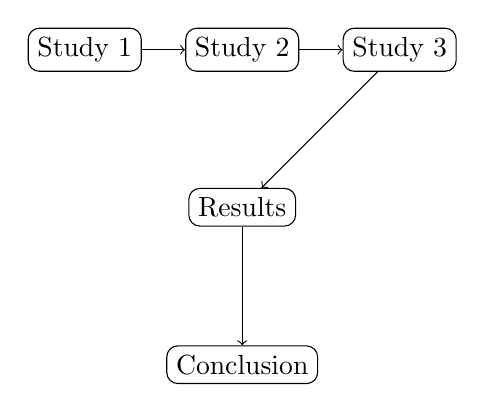
\begin{tikzpicture}[node distance=2cm]
		% Define the nodes
		\node (study1) [draw, rounded corners] {Study 1};
		\node (study2) [right of=study1, draw, rounded corners] {Study 2};
		\node (study3) [right of=study2, draw, rounded corners] {Study 3};
		
		\node (results) [below of=study2, draw, rounded corners] {Results};
		\node (conclusion) [below of=results, draw, rounded corners] {Conclusion};
		
		% Connect the nodes with arrows
		\draw[->] (study1) -- (study2);
		\draw[->] (study2) -- (study3);
		\draw[->] (study3) -- (results);
		\draw[->] (results) -- (conclusion);
	\end{tikzpicture}
	\caption{Flow Diagram of Studies and Results}
\end{figure}




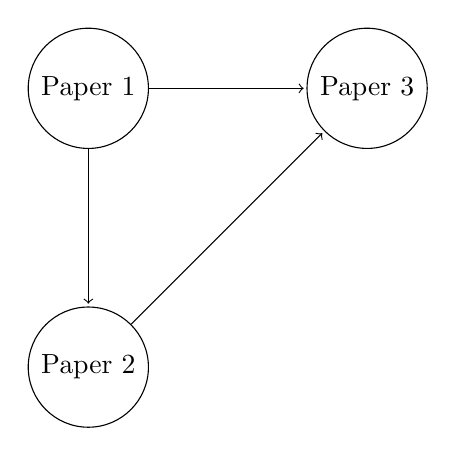
\begin{tikzpicture}[shorten >=1pt, node distance=2cm, auto]
	% Define the nodes (papers)
	\node[draw, circle] (paper1) {Paper 1};
	\node[draw, circle, below=of paper1] (paper2) {Paper 2};
	\node[draw, circle, right=of paper1] (paper3) {Paper 3};
	
	% Define the connections (citations)
	\path[->] (paper1) edge (paper2);
	\path[->] (paper2) edge (paper3);
	\path[->] (paper1) edge (paper3);
\end{tikzpicture}


















\begin{figure*}[ht]
	\centering
	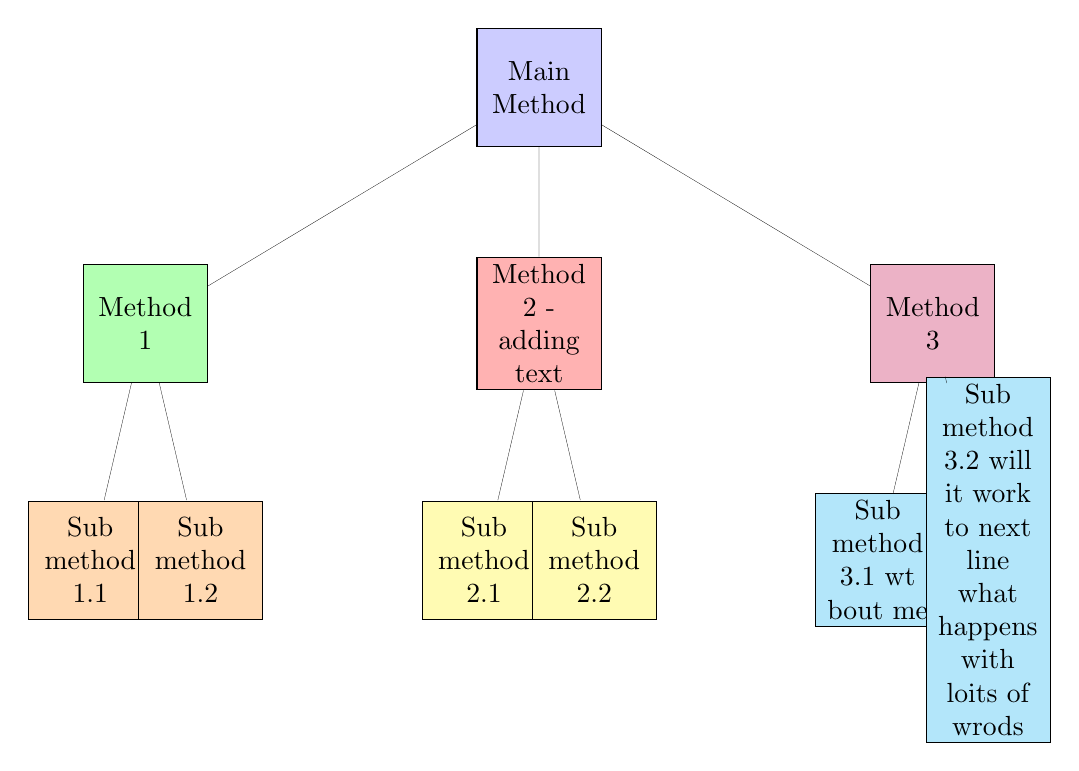
\begin{tikzpicture}[edge from parent/.style={draw, line width=0.1pt, -}, 
		level 1/.style={sibling distance=2.5cm}, % Adjust sibling distance for level 1
		level 2/.style={sibling distance=.7cm}, % Adjust sibling distance for level 2
		level distance=1.5cm,  % Adjust distance between levels
		every node/.style={minimum height=1.5cm, align=center, draw, fill=blue!20, text centered},  % Node styling with larger height
		text width=1.4cm, % Limit text width to avoid overly long nodes
		scale=2, % Adjust scale to fit in two-column layout
		inner sep=2.5pt % Padding within nodes
		]
		% Root node (Main Method)
		\node[draw, fill=blue!20, text centered] {Main Method}
		% First branch level (Methods)
		child { node[draw, fill=green!30, text centered] {Method 1}
			child { node[draw, fill=orange!30, text centered] {Sub method 1.1} }
			child { node[draw, fill=orange!30, text centered] {Sub method 1.2} }
		}
		child { node[draw, fill=red!30, text centered] {Method 2 - adding text}
			child { node[draw, fill=yellow!30, text centered] {Sub method 2.1} }
			child { node[draw, fill=yellow!30, text centered] {Sub method 2.2} }
		}
		child { node[draw, fill=purple!30, text centered] {Method 3}
			child { node[draw, fill=cyan!30, text centered] {Sub method 3.1 wt bout me} }
			child { node[draw, fill=cyan!30, text centered] {Sub method 3.2 will it work to next line what happens with loits of wrods} }
		}
		;
	\end{tikzpicture}
	\caption{Methods Tree Diagram in Literature}
\end{figure*}
























\begin{figure*}[ht]
	\centering
	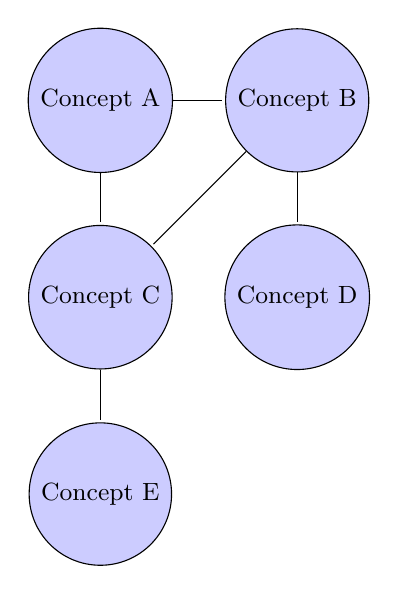
\begin{tikzpicture}[shorten >=1pt, node distance=2.5cm, auto, main node/.style={circle, draw, fill=blue!20, text centered, minimum size=1cm, font=\small}]
		
		% Nodes
		\node[main node] (A) {Concept A};
		\node[main node] (B) [right of=A] {Concept B};
		\node[main node] (C) [below of=A] {Concept C};
		\node[main node] (D) [below of=B] {Concept D};
		\node[main node] (E) [below of=C] {Concept E};
		
		% Edges (connections)
		\path[draw, thin]
		(A) edge (B)
		(A) edge (C)
		(B) edge (D)
		(C) edge (E)
		(B) edge (C);
	\end{tikzpicture}
	\caption{Connected Chart of Methods and Concepts}
\end{figure*}





















































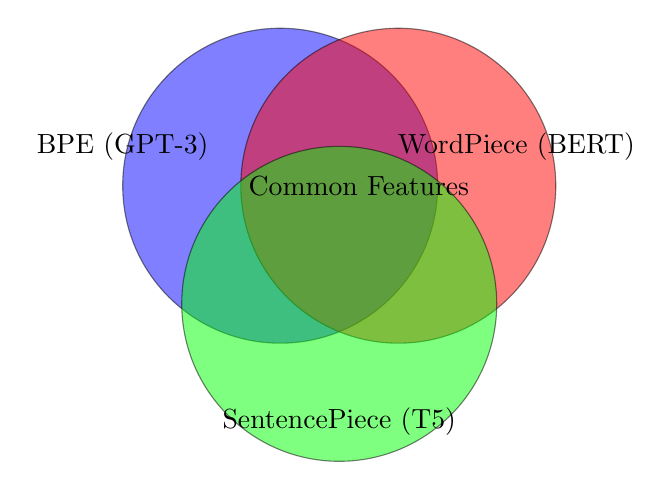
\begin{tikzpicture}
	\draw[fill=blue, opacity=0.5] (0,0) circle(2);
	\draw[fill=red, opacity=0.5] (1.5,0) circle(2);
	\draw[fill=green, opacity=0.5] (0.75,-1.5) circle(2);
	
	\node at (-2, 0.5) {BPE (GPT-3)};
	\node at (3, 0.5) {WordPiece (BERT)};
	\node at (0.75,-3) {SentencePiece (T5)};
	\node at (1, 0) {Common Features};
\end{tikzpicture}


fdfdfdsfas

twat




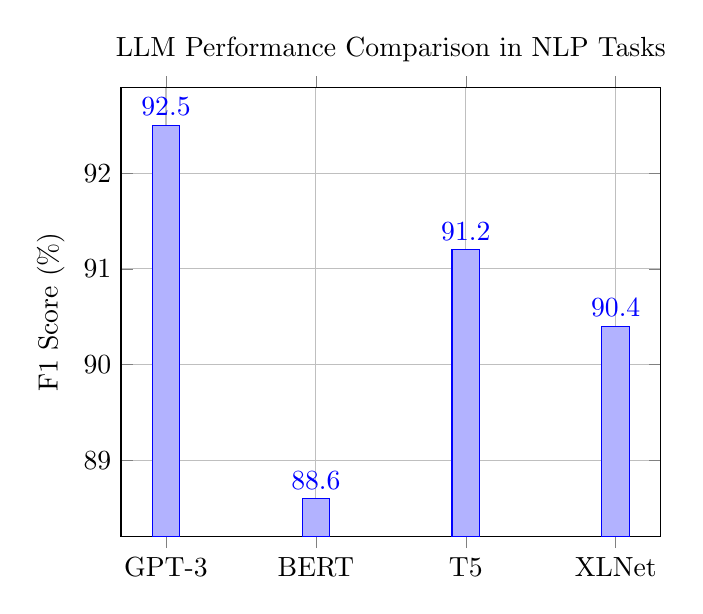
\begin{tikzpicture}
	\begin{axis}[
		ybar,
		symbolic x coords={GPT-3, BERT, T5, XLNet},
		xtick=data,
		ylabel={F1 Score (\%)},
		nodes near coords,
		grid=major,
		title={LLM Performance Comparison in NLP Tasks}
		]
		\addplot coordinates {(GPT-3, 92.5) (BERT, 88.6) (T5, 91.2) (XLNet, 90.4)};
	\end{axis} % This ends the axis environment
\end{tikzpicture} % This ends the tikzpicture environment




fdg gfsgsfg gs ggs

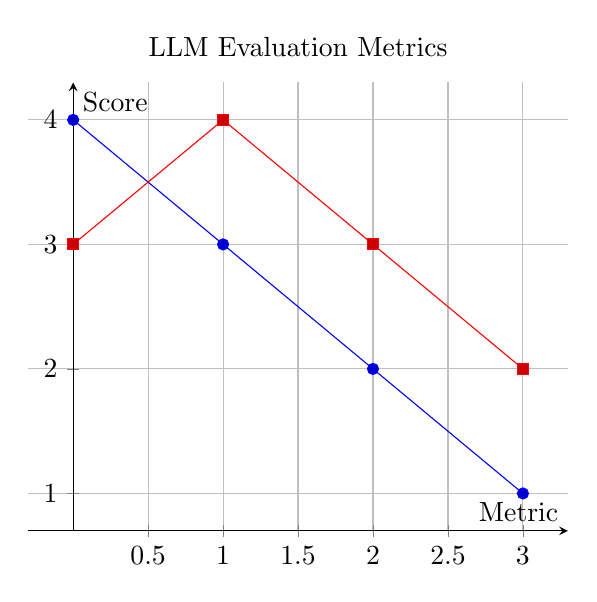
\begin{tikzpicture}
	\begin{axis}[
		axis lines=middle,
		enlargelimits,
		title={LLM Evaluation Metrics},
		ytick={0,1,2,3,4},
		yticklabels={0,1,2,3,4},
		xlabel={Metric},
		ylabel={Score},
		grid=major
		]
		\addplot coordinates {(0, 4) (1, 3) (2, 2) (3, 1)};
		\addplot coordinates {(0, 3) (1, 4) (2, 3) (3, 2)};
	\end{axis}
\end{tikzpicture}



qewq
eq
eqe
qeq



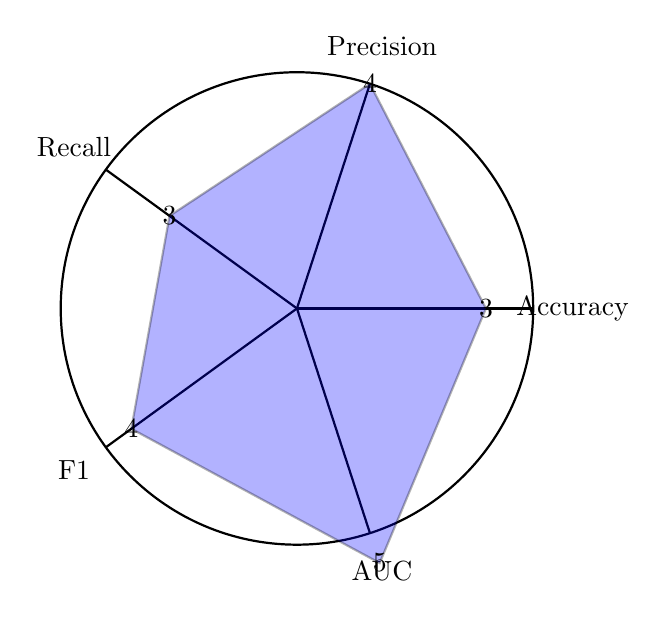
\begin{tikzpicture}
	\draw[thick] (0,0) circle(3); % Draw the outer circle
	\foreach \x in {0, 72, 144, 216, 288} % Coordinates for 5 axes
	\draw[thick] (\x:3) -- (0,0); % Draw axes
	
	% Draw the labels for the axes (Accuracy, Precision, etc.)
	\node at (0:3.5) {Accuracy};
	\node at (72:3.5) {Precision};
	\node at (144:3.5) {Recall};
	\node at (216:3.5) {F1};
	\node at (288:3.5) {AUC};
	
	% Draw the data points and connect them
	\draw[thick, fill=blue, opacity=0.3] 
	(0:2.4) -- 
	(72:3.0) -- 
	(144:2.0) -- 
	(216:2.6) -- 
	(288:3.4) -- cycle;
	
	% Optionally add some labels for each data point
	\node at (0:2.4) {3};
	\node at (72:3.0) {4};
	\node at (144:2.0) {3};
	\node at (216:2.6) {4};
	\node at (288:3.4) {5};
	
\end{tikzpicture}





ffdsfsfsv

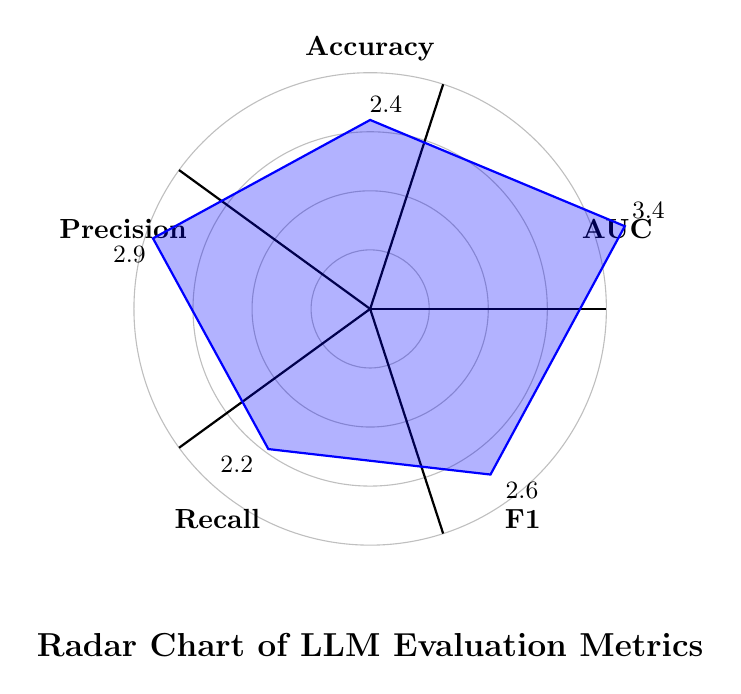
\begin{tikzpicture}
	% Define constants
	\def\n{5}  % Number of axes
	\def\R{3}  % Radius of the radar chart
	
	% Draw concentric circles (grid levels)
	\foreach \i in {1, 2, 3, 4} {
		\draw[gray!50, thin] (0,0) circle (\i * 0.75); % Adjust scaling factor as needed
	}
	
	% Draw axes from center to the boundary
	\foreach \i in {1, 2, ..., \n} {
		\draw[thick] (360/\n * \i:\R) -- (0,0); % Axis lines
	}
	
	% Add axis labels
	\node at (90:\R+0.3) {\textbf{Accuracy}};
	\node at (162:\R+0.3) {\textbf{Precision}};
	\node at (234:\R+0.3) {\textbf{Recall}};
	\node at (306:\R+0.3) {\textbf{F1}};
	\node at (18:\R+0.3) {\textbf{AUC}};
	
	% Define data points (example values for each metric)
	\coordinate (A) at (90:2.4);  % Accuracy
	\coordinate (B) at (162:2.9); % Precision
	\coordinate (C) at (234:2.2); % Recall
	\coordinate (D) at (306:2.6); % F1
	\coordinate (E) at (18:3.4);  % AUC
	
	% Draw filled polygon (data region)
	\fill[blue, opacity=0.3] (A) -- (B) -- (C) -- (D) -- (E) -- cycle;
	
	% Connect data points with a closed path
	\draw[thick, blue] (A) -- (B) -- (C) -- (D) -- (E) -- cycle;
	

	
	% Add values near each data point
	\node[font=\small] at ($(A) + (0.2, 0.2)$) {2.4};
	\node[font=\small] at ($(B) + (-0.3, -0.2)$) {2.9};
	\node[font=\small] at ($(C) + (-0.4, -0.2)$) {2.2};
	\node[font=\small] at ($(D) + (0.4, -0.2)$) {2.6};
	\node[font=\small] at ($(E) + (0.3, 0.2)$) {3.4};
	
	% Title below the chart
	\node[below=1cm, align=center, font=\large\bfseries] at (0,-\R) {Radar Chart of LLM Evaluation Metrics};
	
\end{tikzpicture}

gsgdsgsdg



small heatmap


affaf
ar
ara
ra
rar
a
\begin{figure}[h]
\centering
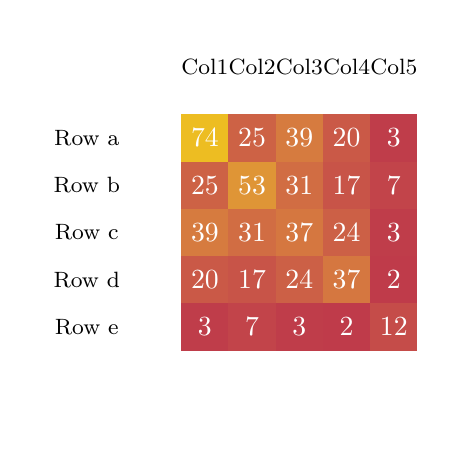
\begin{tikzpicture}[scale=.6]
	\foreach \y [count=\n] in {
		{74,25,39,20,3},
		{25,53,31,17,7},
		{39,31,37,24,3},
		{20,17,24,37,2},
		{3,7,3,2,12},
	} {

		% heatmap tiles
		\foreach \x [count=\m] in \y {
			\node[fill=yellow!\x!purple, minimum size=6mm, text=white] at (\m,-\n) {\x};
		}
	}
	
	% row labels
	\foreach \a [count=\i] in {Row a,Row b,Row c,Row d,Row e,} {
		\node[minimum size=15mm, font=\footnotesize] at (-1.5,-\i) {\a};
	}
	
	% Column labels (custom)
	\foreach \b [count=\j] in {Col1, Col2, Col3, Col4, Col5} {
		\node[minimum size=10mm, font=\footnotesize] at (\j,  0.5) {\b};

				 % Custom column labels
	}
	
	
\end{tikzpicture}
\caption{5x5 Heatmap Example}
\label{fig:heatmap}
\end{figure}
















\subsection{Abbreviations and Acronyms}\label{AA}
Define abbreviations and acronyms the first time they are used in the text, 
even after they have been defined in the abstract. Abbreviations such as 
IEEE, SI, MKS, CGS, ac, dc, and rms do not have to be defined. Do not use 
abbreviations in the title or heads unless they are unavoidable.

\subsection{Units}
\begin{itemize}
\item Use either SI (MKS) or CGS as primary units. (SI units are encouraged.) English units may be used as secondary units (in parentheses). An exception would be the use of English units as identifiers in trade, such as ``3.5-inch disk drive''.
\item Avoid combining SI and CGS units, such as current in amperes and magnetic field in oersteds. This often leads to confusion because equations do not balance dimensionally. If you must use mixed units, clearly state the units for each quantity that you use in an equation.
\item Do not mix complete spellings and abbreviations of units: ``Wb/m\textsuperscript{2}'' or ``webers per square meter'', not ``webers/m\textsuperscript{2}''. Spell out units when they appear in text: ``. . . a few henries'', not ``. . . a few H''.
\item Use a zero before decimal points: ``0.25'', not ``.25''. Use ``cm\textsuperscript{3}'', not ``cc''.)
\end{itemize}

\subsection{Equations}
Number equations consecutively. To make your 
equations more compact, you may use the solidus (~/~), the exp function, or 
appropriate exponents. Italicize Roman symbols for quantities and variables, 
but not Greek symbols. Use a long dash rather than a hyphen for a minus 
sign. Punctuate equations with commas or periods when they are part of a 
sentence, as in:
\begin{equation}
a+b=\gamma\label{eq}
\end{equation}

Be sure that the 
symbols in your equation have been defined before or immediately following 
the equation. Use ``\eqref{eq}'', not ``Eq.~\eqref{eq}'' or ``equation \eqref{eq}'', except at 
the beginning of a sentence: ``Equation \eqref{eq} is . . .''

\subsection{\LaTeX-Specific Advice}

Please use ``soft'' (e.g., \verb|\eqref{Eq}|) cross references instead
of ``hard'' references (e.g., \verb|(1)|). That will make it possible
to combine sections, add equations, or change the order of figures or
citations without having to go through the file line by line.

Please don't use the \verb|{eqnarray}| equation environment. Use
\verb|{align}| or \verb|{IEEEeqnarray}| instead. The \verb|{eqnarray}|
environment leaves unsightly spaces around relation symbols.

Please note that the \verb|{subequations}| environment in {\LaTeX}
will increment the main equation counter even when there are no
equation numbers displayed. If you forget that, you might write an
article in which the equation numbers skip from (17) to (20), causing
the copy editors to wonder if you've discovered a new method of
counting.


{\LaTeX} can't read your mind. If you assign the same label to a
subsubsection and a table, you might find that Table I has been cross
referenced as Table IV-B3. 

{\LaTeX} does not have precognitive abilities. If you put a
\verb|\label| command before the command that updates the counter it's
supposed to be using, the label will pick up the last counter to be
cross referenced instead. In particular, a \verb|\label| command
should not go before the caption of a figure or a table.

Do not use \verb|\nonumber| inside the \verb|{array}| environment. It
will not stop equation numbers inside \verb|{array}| (there won't be
any anyway) and it might stop a wanted equation number in the
surrounding equation.



\subsection{Figures and Tables}\label{FAT}
\paragraph{Positioning Figures and Tables} Place figures and tables at the top and 
bottom of columns. Avoid placing them in the middle of columns. Large 
figures and tables may span across both columns. Figure captions should be 
below the figures; table heads should appear above the tables. Insert 
figures and tables after they are cited in the text. Use the abbreviation 
``Fig.~\ref{fig}'', even at the beginning of a sentence.

\begin{table}[htbp]
\caption{Table Type Styles}
\begin{center}
\begin{tabular}{|c|c|c|c|}
\hline
\textbf{Table}&\multicolumn{3}{|c|}{\textbf{Table Column Head}} \\
\cline{2-4} 
\textbf{Head} & \textbf{\textit{Table column subhead}}& \textbf{\textit{Subhead}}& \textbf{\textit{Subhead}} \\
\hline
copy& More table copy$^{\mathrm{a}}$& &  \\
\hline
\multicolumn{4}{l}{$^{\mathrm{a}}$Sample of a Table footnote.}
\end{tabular}
\label{tab1}
\end{center}
\end{table}

\begin{figure}[htbp]
\centerline{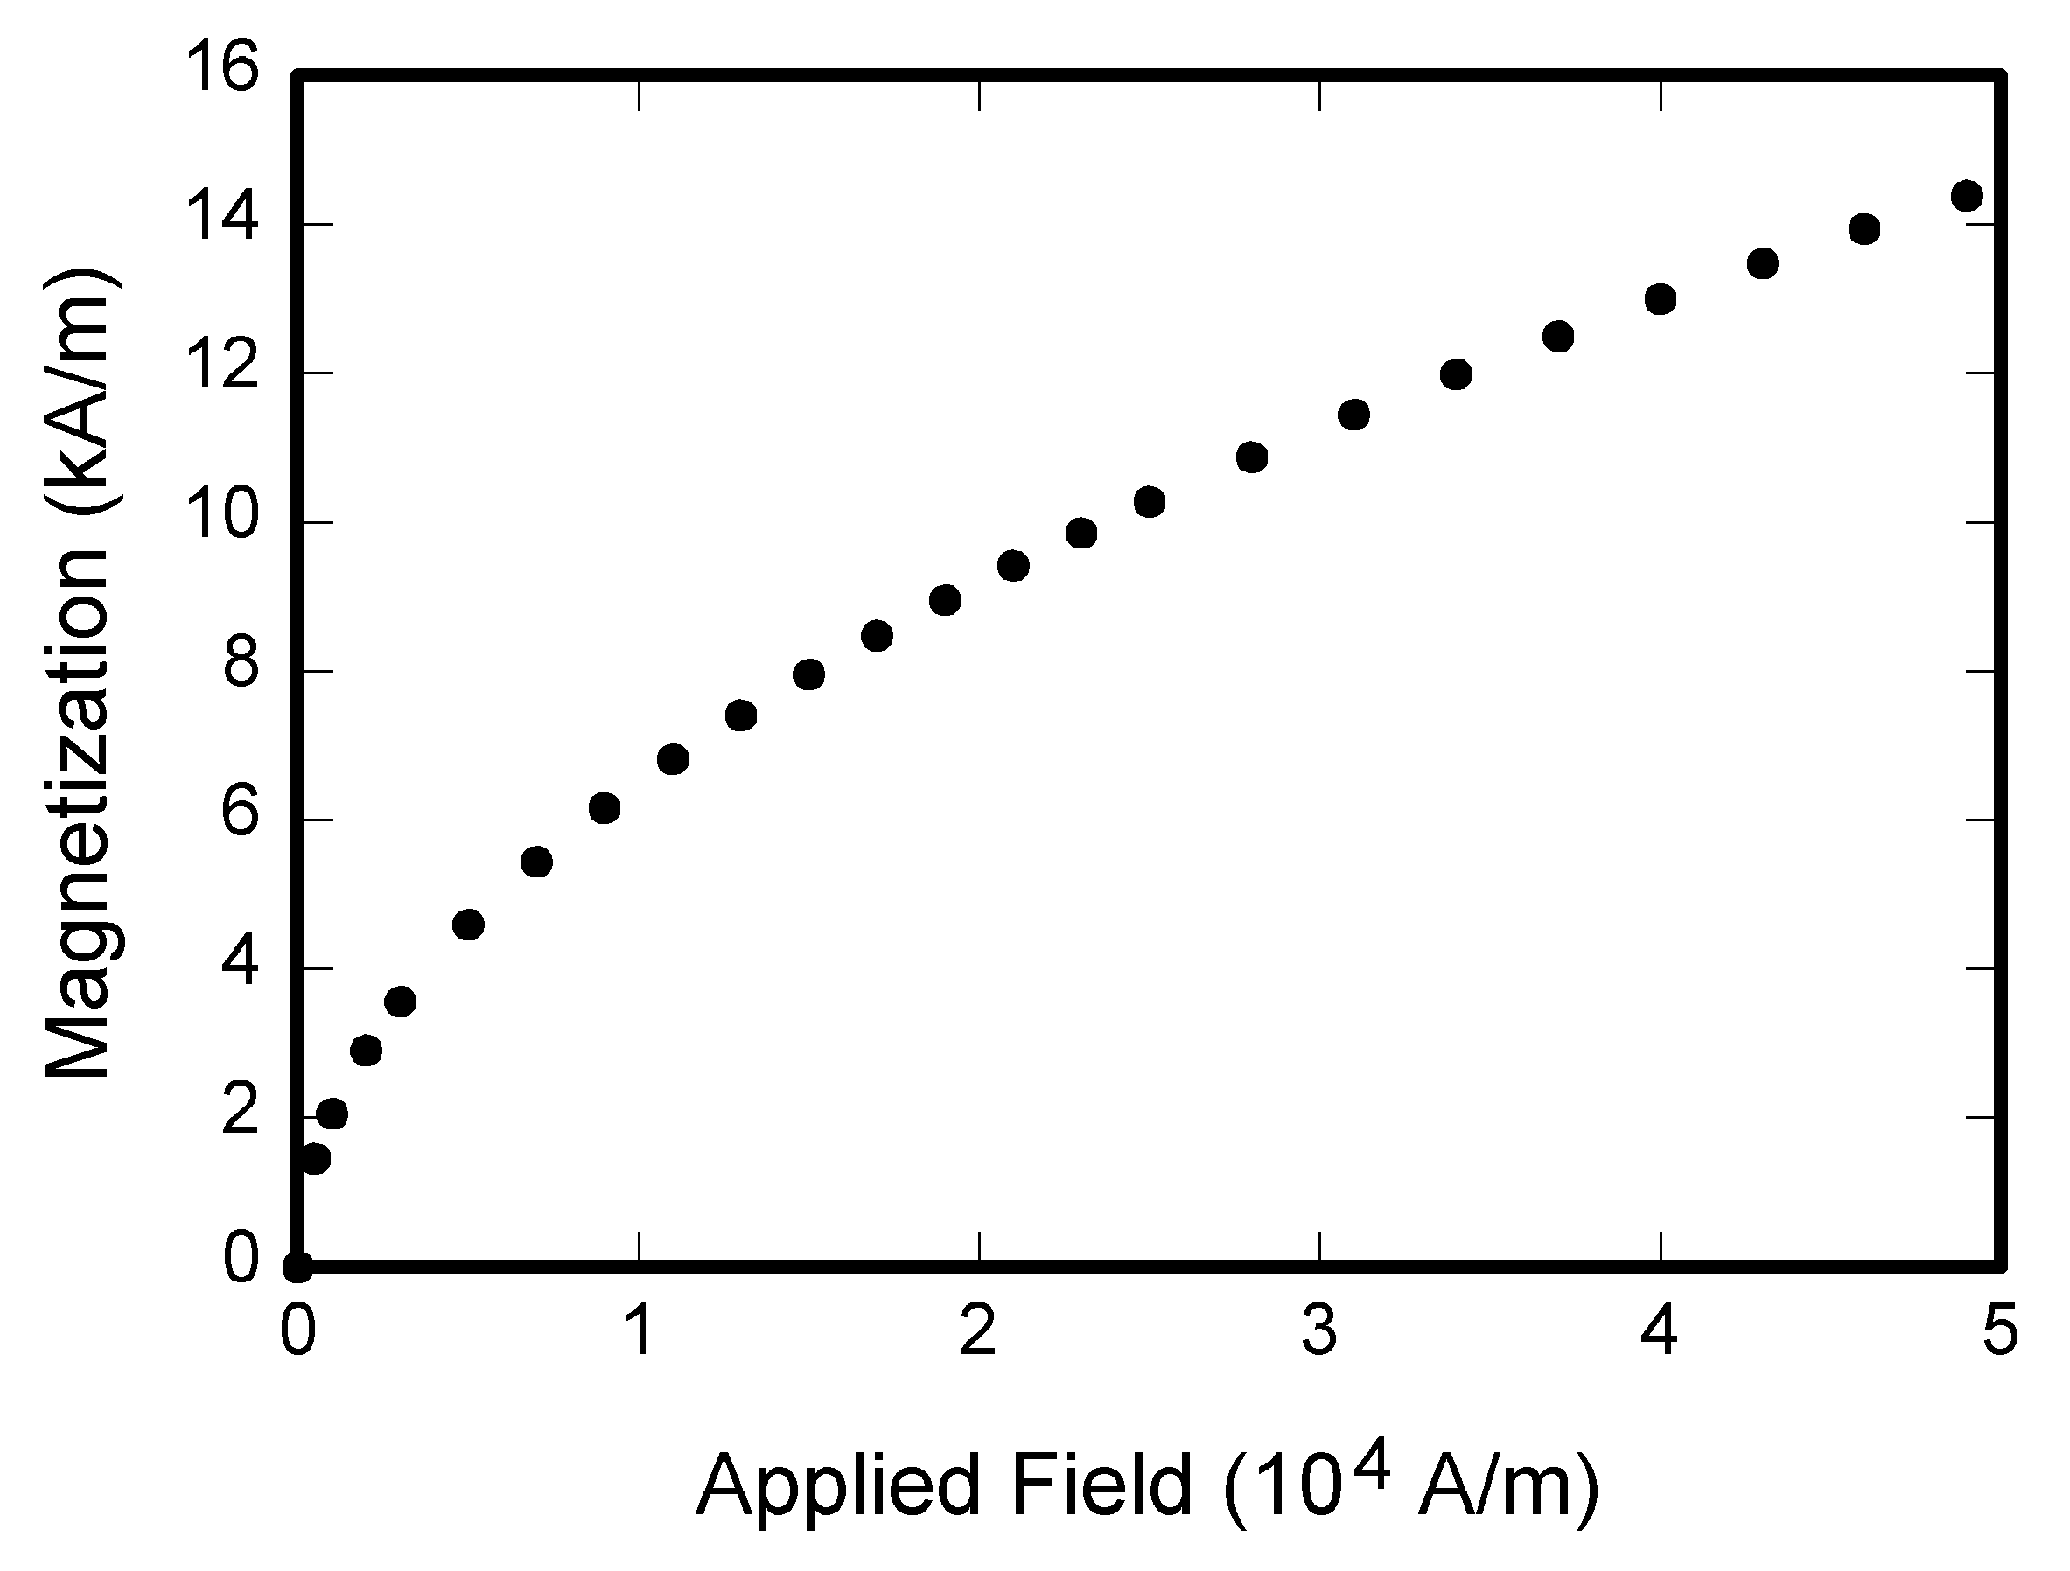
\includegraphics{fig1.png}}
\caption{Example of a figure caption.}
\label{fig}
\end{figure}

Figure Labels: Use 8 point Times New Roman for Figure labels. Use words 
rather than symbols or abbreviations when writing Figure axis labels to 
avoid confusing the reader. As an example, write the quantity 
``Magnetization'', or ``Magnetization, M'', not just ``M''. If including 
units in the label, present them within parentheses. Do not label axes only 
with units. In the example, write ``Magnetization (A/m)'' or ``Magnetization 
\{A[m(1)]\}'', not just ``A/m''. Do not label axes with a ratio of 
quantities and units. For example, write ``Temperature (K)'', not 
``Temperature/K''.


\section{Proposed Methodology}
We propose to integrate like code assist, model assist to the modeling framework to ease developing regulating and testing models.

\section{Conclusion}

We have proposed on the optimal way to integrate current Gen Ai in risk modeling.


\section*{Acknowledgment}

The preferred spelling of the word ``acknowledgment'' in America is without 
an ``e'' after the ``g''. Avoid the stilted expression ``one of us (R. B. 
G.) thanks $\ldots$''. Instead, try ``R. B. G. thanks$\ldots$''. Put sponsor 
acknowledgments in the unnumbered footnote on the first page.





\printbibliography  % Print the reference list



\vspace{12pt}
\color{red}
IEEE conference templates contain guidance text for composing and formatting conference papers. Please ensure that all template text is removed from your conference paper prior to submission to the conference. Failure to remove the template text from your paper may result in your paper not being published.




















\end{document}
